\documentclass[12pt,a4paper,final]{article}
\usepackage[left=2.5cm,right=2.5cm,top=2.5cm,bottom=2.5cm]{geometry}

%% IDIOMA
\usepackage[utf8]{inputenc}
\usepackage[portuguese]{babel}

%% TRANSFORMAÇÕES ESTILO CSS
\usepackage{graphicx}

%% ESTÉTICA
\usepackage{enumerate}
\usepackage{booktabs}
\usepackage{amsmath, amsthm, amssymb, amsfonts}
\usepackage{multirow}
\usepackage[hyphens]{url}
\usepackage{subfig}

%% FONTE
\usepackage[T1]{fontenc}
%\usepackage[sc]{mathpazo} % Palatino with smallcaps
\usepackage{mathptmx}
\usepackage{eulervm} % Euler math

%% TIPOGRAFIA
\usepackage{parskip}
\usepackage[activate={true,nocompatibility},final,tracking=true,kerning=true,spacing=true,factor=1100,stretch=10,shrink=10]{microtype}

%% CODIGO
\usepackage{listings}
\usepackage{color}

\definecolor{dkgreen}{rgb}{0,0.6,0}
\definecolor{gray}{rgb}{0.5,0.5,0.5}
\definecolor{mauve}{rgb}{0.58,0,0.82}

\lstset{frame=tb,
  aboveskip=3mm,
  belowskip=3mm,
  showstringspaces=false,
  columns=flexible,
  basicstyle={\small\ttfamily},
  numbers=none,
  numberstyle=\tiny\color{gray},
  keywordstyle=\color{blue},
  commentstyle=\color{dkgreen},
  stringstyle=\color{mauve},
  breaklines=true,
  breakatwhitespace=true,
  tabsize=3
}

\title{Relatório 6 de TCC2/IC}
\author{Ly Sandro Amorim de Campos Salles\\Departamento de Física\\Universidade Federal do Paraná}
\date{\today}

\begin{document}
	\maketitle

  Desde o último encontro foram feitos alguns avanços no desenvolvimento do novo programa de simulações de autômatos celulares. Resumidamente:
  \begin{enumerate}
    \item A reescrita do que já havia sido feito para entrar em conformidade com o plano de desenvolvimento apresentado no relatório anterior;
    \item A criação de um menu (\textit{front-end}) para as simulações;
    \item A reescrita do Inhomogenous Cellular Automata de Gerard Weisbuch e Dietrich Stauffer;
    \item A implementação do algoritmo de contagem de aglomerados por ``contaminação'';
  \end{enumerate}
  Detalhadamente:\\
\texttt{\small
Thu Apr 4 15:38:33 2019 -0300 by Ly Sandro: CAmanager updated to print number of clusters\\
Thu Apr 4 15:37:53 2019 -0300 by Ly Sandro: ICA.c now counts clusters\\
Wed Apr 3 13:57:00 2019 -0300 by Ly Sandro: improved maintenance costs of makefile\\
Wed Apr 3 13:52:24 2019 -0300 by Ly Sandro: fixed output in startSimulation()\\
Wed Apr 3 13:50:18 2019 -0300 by Ly Sandro: fixed ICA\_neighborSum giving wrong aswer\\
Wed Apr 3 12:38:48 2019 -0300 by Ly Sandro: fixed segmentation fault in ICA.c\\
Tue Apr 2 18:46:30 2019 -0300 by Ly Sandro: added new functions to ICA.c\\
Tue Apr 2 18:45:14 2019 -0300 by Ly Sandro: added some test procedures to CAmanager.c\\
Tue Apr 2 18:44:40 2019 -0300 by Ly Sandro: updated makefile to include new files\\
Tue Apr 2 18:44:10 2019 -0300 by Ly Sandro: INCLUDED NEW FUNCTIONS IN ica.H\\
Tue Apr 2 00:35:18 2019 -0300 by Ly Sandro: created CAmanager\\
Tue Apr 2 00:35:01 2019 -0300 by Ly Sandro: added a CA manager to optionManager\\
Tue Apr 2 00:33:20 2019 -0300 by Ly Sandro: ICA rewritten\\
Mon Apr 1 18:26:14 2019 -0300 by Ly Sandro: listOptions made more compact\\
Mon Apr 1 18:21:29 2019 -0300 by Ly Sandro: printTitle is now 1 line more compact\\
Mon Apr 1 18:18:47 2019 -0300 by Ly Sandro: Improved CAexplorer.c main function's output readability\\
Mon Apr 1 18:00:55 2019 -0300 by Ly Sandro: makefile updated to include the menu option manager\\
Mon Apr 1 17:56:22 2019 -0300 by Ly Sandro: menu option manager created\\
Mon Apr 1 17:55:03 2019 -0300 by Ly Sandro: CAexplorer.c's main function now uses a menu option manager\\
Mon Apr 1 13:56:02 2019 -0300 by Ly Sandro: Added function description in printTitle.h\\
Mon Apr 1 13:55:05 2019 -0300 by Ly Sandro: Improved functions' storage classes\\
Mon Apr 1 13:49:43 2019 -0300 by Ly Sandro: Included vscode folder to gitignore\\
Thu Mar 7 18:15:33 2019 -0300 by Ly Sandro: Files reorganized for better program management\\
}

Essas informações e o código desenvolvido podem ser visualizados em \url{https://github.com/Ly54ndr0/CellularAutomataExplorer}.

Essa nova versão já tem as mesmas capacidades da antiga versão do programa de simulações de InCA's, além de estar mais rápida e melhor organizada. Abaixo estão alguns gráficos relizados com dados obtidos através do novo programa.

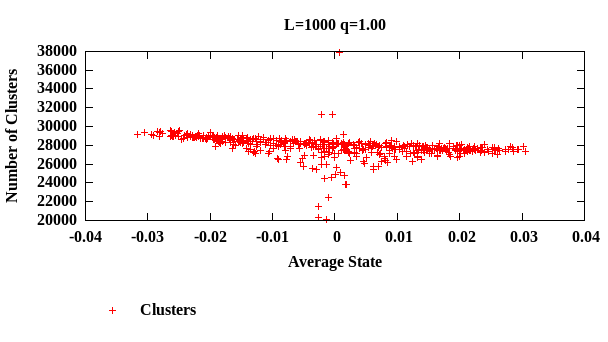
\includegraphics[width=\linewidth]{dataL1000Q100ClustersVsAvgState.png}

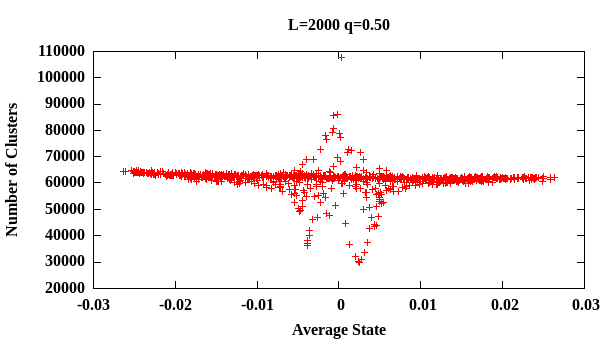
\includegraphics[width=\linewidth]{dataL2000Q50ClustersVsAvgState.png}

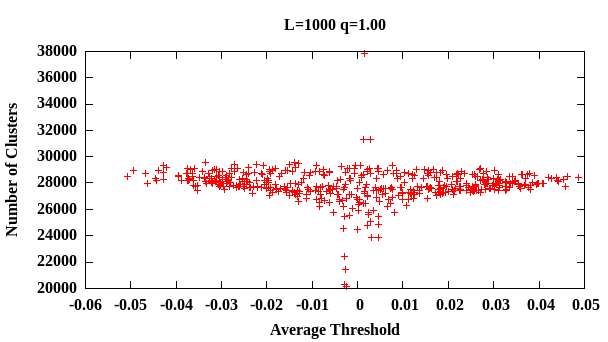
\includegraphics[width=\linewidth]{dataL1000Q100ClustersVsAvgThres.png}

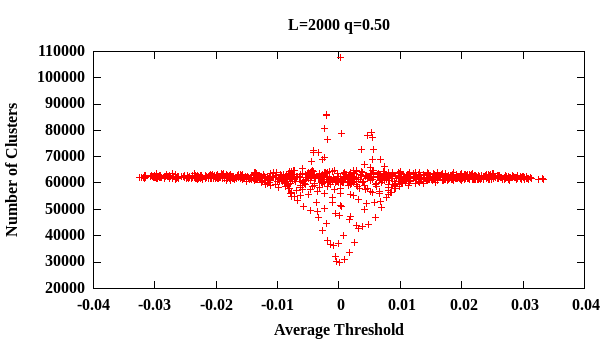
\includegraphics[width=\linewidth]{dataL2000Q50ClustersVsAvgThres.png}

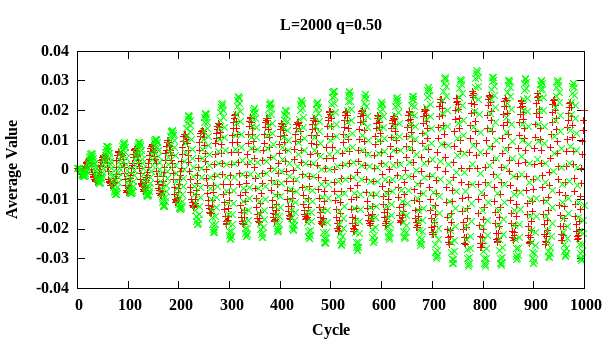
\includegraphics[width=\linewidth]{dataL2000Q50AvgStateThresVScycle.png}\\
Neste último gráfico o limiar médio está em verde e em vermelho está o estado médio.

Os gráficos com $L=1000$ têm 500 pontos de dados.
Os gráficos com $L=2000$ têm 1000 pontos de dados.

  Para os próximos dias, estas serão as tarefas realizadas:
	\begin{enumerate}
		\item A finalização do novo programa de simulações de autômatos celulares;
		\item Verificação da sopreposição da curva do potencial de Lennard-Jones no gráfico de afinidade em função de $q$.
		\item Leitura do artigo ``Stochastic Cellular Automata Model for Stock Market Dynamics'' dos autores M. Bartolozzi e A. W. Thomas;
		\item Pesquisa sobre como a volatilidade de mercado influencia na aglomeração dos agentes;
		\item A leitura do Capítulo 4 (``Nonlinear Oscillations and Chaos'') do livro ``Classical Dynamics of Particles and Systems'' dos autores Stephen T. Thornton e Jerry B. Marion.
	\end{enumerate}

\end{document}
